% =============================================================================
% RELATORIO N1 - INTELIGENCIA ARTIFICIAL - 7N CC - NOITE
% Universidade Presbiteriana Mackenzie
% Prof. Dr. Ivan Carlos Alcantara de Oliveira
%
% Historico de alteracoes:
% 2026-03-28 | Grupo B3-LSTM | Criacao do documento inicial
% =============================================================================

\documentclass[12pt]{article}

\usepackage[T1]{fontenc}		% Codificacao de saída das fontes (define \normalsfcodes)
\usepackage[utf8]{inputenc}		% Codificacao do documento
\usepackage{sbc-template}
\usepackage{indentfirst}		
\usepackage{graphicx,url}
\usepackage{microtype} 			% Para melhorias de justificação
\usepackage[brazilian]{babel}
\usepackage{booktabs}
\usepackage{array}
\usepackage{amsmath}
\usepackage{amssymb}

\sloppy

% Correcao de compatibilidade: sbc-template.sty redefine \normalsize sem
% incluir \normalsfcodes; o kernel LaTeX 2025+ chama \normalsfcodes
% diretamente em \@outputpage e em hooks do babel, causando
% "Undefined control sequence". Restauramos \normalsfcodes apos o template.
\makeatletter
\def\normalsfcodes{\sfcode`\.=\@m}
\makeatother

% Macro de fonte para figuras e tabelas (NBR 14724)
\newcommand{\fonte}[1]{\par\vspace{-0.2em}{\footnotesize\textit{Fonte: #1}}\par}

% =============================================================================
% PREENCHA OS CAMPOS ABAIXO COM OS DADOS DO GRUPO
% ATENCAO: nao use colchetes [ ] nos campos \author e \address pois
% o tabular interno do SBC os interpreta como argumento opcional de \\.
% Use apenas texto simples ou comandos LaTeX validos.
% =============================================================================
% TITULO: pode usar acentos normalmente (UTF-8)
\title{Previsão do preço futuro da ação ITUB4\\
       Utilizando Redes Neurais Recorrentes do Tipo LSTM}

% AUTORES: substitua pelos nomes reais.
% ATENCAO: NAO use colchetes [ ] aqui. O tabular interno do SBC
% interpretaria [ ] apos \\ como argumento de espacamento e causaria erro.
% Use \inst{1} para o numero de afiliacao e \\ para quebrar linha entre autores.
\author{Gabriel Alves de F Spinola Sucupira\inst{1} \and Henrique Pena Ribeiro\inst{1}\\
        Lucas Zanini da Silva\inst{1} \and Tiago Teraoka e Sá \inst{1}}

% ENDERECO / E-MAILS: substitua pelos e-mails reais.
% ATENCAO: NAO use \\ dentro de \email{}. Separe os e-mails por virgula
% em sequencia continua -- o \\ dentro de \email causaria o mesmo erro acima.
\address{Faculdade de Computação e Informática --
  Universidade Presbiteriana Mackenzie \\}


% =============================================================================
\begin{document}

\maketitle

% ---------------------------------------------------------------------------
\begin{resumo}
A bolsa de valores brasileira (B3) registrou crescimento de 23\% no número
de investidores pessoas físicas em 2023, ampliando a demanda por ferramentas
de apoio à tomada de decisão. Este documento apresenta os resultados parciais
de um projeto que aplica uma rede neural recorrente do tipo LSTM
(\textit{Long Short-Term Memory}) de camada única para a previsão do preço
de fechamento do ativo ITUB4 (Itaú Unibanco) na B3 com horizonte de um dia.
Os dados históricos dos últimos 5 anos são coletados via API
\textit{yfinance}, utilizando abertura, máxima, mínima, fechamento,
volume e Média Móvel Exponencial de 60 dias (EMA-60) como variáveis
preditoras. Os dados são normalizados via Z-score e organizados em janelas
temporais de 50 dias, com divisão cronológica em treino e teste
(80\%/20\%). Um modelo de persistência é implementado como
\textit{baseline} de comparação. A avaliação utilizará as métricas RMSE,
MAE e MAPE. Como resultado esperado, o modelo deve superar o
\textit{baseline} e ser integrado em uma aplicação web interativa
desenvolvida com Streamlit.

\vspace{0.5em}\noindent\textbf{Palavras-chave:} LSTM; previsão de preços
de ações; redes neurais recorrentes; B3; ITUB4; séries temporais.
\end{resumo}

\begin{abstract}
The Brazilian stock exchange (B3) has seen a 23\% growth in individual
investors in 2023, creating demand for analytical tools to support
decision-making. This paper presents the partial results of a project that
applies a single-layer Long Short-Term Memory (LSTM) neural network for
one-day-ahead closing price prediction of the ITUB4 stock (Itaú Unibanco)
on the B3. Historical data from the past 5 years is collected via the
\textit{yfinance} API, covering Open, High, Low, Close, Volume, and
a 60-day Exponential Moving Average (EMA-60) as features. Data is
standardized with Z-score normalization and structured into 50-day temporal
windows with a chronological train/test split (80\%/20\%).
A persistence model is implemented as a baseline. Performance will be
evaluated using RMSE, MAE, and MAPE metrics. The expected outcome is
a model that consistently outperforms the baseline and serves as the backend
for an interactive Streamlit web application.

\vspace{0.5em}\noindent\textbf{Keywords:} LSTM; stock price prediction;
recurrent neural networks; B3; ITUB4; time series forecasting.
\end{abstract}

% ===========================================================================
\section{Introdução}
% ===========================================================================

\subsection{Contextualização}

O mercado de capitais brasileiro, operado pela B3 (Brasil, Bolsa e Balcão),
tem vivenciado crescimento expressivo na última década. Segundo dados da
própria bolsa, o número de investidores pessoas físicas cresceu 23\% em 2023,
ampliando significativamente a base de participantes do mercado acionário
nacional. Esse crescimento, no entanto, não é acompanhado proporcionalmente
pela capacitação técnica dos novos investidores, muitos dos quais ingressam
sem o embasamento necessário para análise fundamentalista ou técnica dos
ativos \cite{zanotto:2026}.

O comportamento dos preços de ações é determinado por uma complexa
combinação de fatores: indicadores técnicos derivados do histórico de preços,
variáveis macroeconômicas (taxa de juros, inflação, câmbio), resultados
financeiros das empresas e eventos externos de caráter político ou
geopolítico. A análise manual e integrada de todos esses fatores ultrapassa
a capacidade operacional da maioria dos investidores individuais, criando
espaço para soluções baseadas em Inteligência Artificial (IA) que consigam
extrair padrões significativos de séries históricas.

\subsection{Justificativa}

Modelos clássicos de séries temporais, como o ARIMA, assumem linearidade e
estacionariedade nos dados, premissas raramente satisfeitas em séries
financeiras reais \cite{box:1970}. Redes neurais recorrentes do tipo LSTM
(\textit{Long Short-Term Memory}), propostas por
\cite{hochreiter:1997}, foram projetadas especificamente para aprender dependências temporais
de longo prazo em dados sequenciais não-lineares, tornando-as candidatas
naturais para a previsão de preços de ativos financeiros.

A revisão sistemática de \cite{mintarya:2023} confirma que a adoção de
LSTM em aplicações financeiras cresceu de forma consistente a partir de 2015,
superando abordagens como SVM e redes neurais convencionais. No contexto
específico da B3, estudos como os de \cite{silveira:2021} e
\cite{zanotto:2026} demonstram a viabilidade e a eficácia dessa arquitetura
para previsão de ativos brasileiros, área com menor cobertura na literatura
do que bolsas internacionais como a NYSE ou a bolsa de Xangai.

\subsection{Objetivo}

O objetivo geral deste projeto é desenvolver, treinar e validar um modelo
LSTM de camada única para prever o preço de fechamento do ativo ITUB4
(Itaú Unibanco S.A.) na B3 com antecedência de um dia útil, utilizando
dados históricos de preços e indicadores técnicos derivados. Como objetivos
específicos, destacam-se:

\begin{itemize}
  \item Coletar e preparar uma série histórica de 5 anos do ativo ITUB4
        via API \textit{yfinance} (Open, High, Low, Close, Volume);
  \item Realizar análise exploratória dos dados com gráficos de preço,
        volume, retornos, médias móveis, correlações e identificação visual
        de tendência, sazonalidade e períodos atípicos;
  \item Implementar um modelo de persistência como \textit{baseline} de
        comparação;
  \item Construir e treinar o modelo LSTM com 150 neurônios, avaliando seu
        desempenho frente ao \textit{baseline} pelas métricas RMSE, MAE
        e MAPE;
  \item Desenvolver um protótipo web com Streamlit para visualização
        interativa das previsões e comunicação das limitações do modelo.
\end{itemize}

\subsection{Opção do Projeto}

Este projeto enquadra-se na \textbf{Opção ML/DL} (Machine Learning / Deep
Learning), conforme as diretrizes da disciplina, empregando uma rede neural
LSTM para solucionar um problema de regressão/predição em série temporal
financeira, com dados capturados pelo grupo via API pública.


% ===========================================================================
\section{Fundamentação Teórica}
% ===========================================================================

\subsection{Modelos Clássicos de Séries Temporais}

A modelagem de séries temporais financeiras tem longa tradição acadêmica. O
modelo ARIMA (\textit{Auto-Regressive Integrated Moving Average}), introduzido
por \cite{box:1970} na década de 1970, foi por décadas o padrão de referência
para previsão de séries univariadas. O ARIMA combina
autorregressão (AR), diferenciação para tornar a série estacionária (I) e
médias móveis dos resíduos (MA). Suas principais limitações para aplicação
em dados financeiros são: (i) exigência de estacionariedade, que requer
transformações que podem comprometer a estrutura e interpretabilidade dos
dados; e (ii) incapacidade de capturar relações não-lineares, frequentes em
séries de preços de ativos \cite{nascimento:2022}.

\subsection{Redes Neurais Recorrentes (RNN)}

Redes neurais artificiais convencionais (\textit{feedforward}) processam cada
entrada de forma independente, sem memória de passos anteriores, tornando-as
inadequadas para dados sequenciais. As Redes Neurais Recorrentes (RNN)
introduzem conexões cíclicas que permitem a passagem de informação entre
instantes de tempo consecutivos, habilitando o aprendizado de dependências
temporais. O treinamento ocorre via retropropagação através do tempo
(\textit{Backpropagation Through Time} -- BPTT). Contudo, em sequências longas,
os gradientes tendem a decair exponencialmente nas camadas anteriores, problema conhecido como \textit{vanishing gradient}, impedindo que a rede
aprenda dependências de longo prazo.

\subsection{LSTM (\textit{Long Short-Term Memory})}

A arquitetura LSTM, proposta por \cite{hochreiter:1997}, resolve o
\textit{vanishing gradient} mediante um mecanismo de portões (\textit{gates})
e um componente chamado \textbf{estado da célula} ($c_t$), que mantém um
caminho linear ao longo do tempo com operações de soma e multiplicação simples,
preservando o fluxo de gradientes sem ativações não-lineares que causariam
decaimento.

Cada célula LSTM recebe, a cada instante $t$: a entrada atual $x_t$, o estado
oculto anterior $h_{t-1}$ (memória de curto prazo) e o estado da célula
anterior $c_{t-1}$ (memória de longo prazo). Três portões controlam
seletivamente o fluxo de informações:

\begin{itemize}
  \item \textbf{Forget gate}: decide quais informações de $c_{t-1}$ devem ser
        descartadas -- $f_t = \sigma(W_f x_t + W_{hf} h_{t-1} + b_f)$;
  \item \textbf{Input gate}: decide quais novas informações serão armazenadas
        -- $i_t = \sigma(W_i x_t + W_{hi} h_{t-1} + b_i)$;
  \item \textbf{Output gate}: decide quais informações do estado atual serão
        passadas como saída -- $o_t = \sigma(W_o x_t + W_{ho} h_{t-1} + b_o)$.
\end{itemize}

O estado da célula é atualizado por $c_t = f_t \otimes c_{t-1} + i_t \otimes
\tilde{c}_t$, onde $\tilde{c}_t = \tanh(W_c x_t + W_{hc} h_{t-1} + b_c)$.
O estado oculto de saída é dado por $h_t = o_t \otimes \tanh(c_t)$, onde
$\sigma$ é a função sigmoide, $\tanh$ é a tangente hiperbólica e $\otimes$
é o produto elemento a elemento.

\subsection{Média Móvel Exponencial (EMA)}

A Média Móvel Exponencial (\textit{Exponential Moving Average} -- EMA) é um
indicador técnico de tendência que pondera as observações históricas de forma
exponencialmente decrescente, atribuindo maior peso aos preços mais recentes.
Diferentemente da Média Móvel Simples (SMA), que trata todas as observações
da janela com pesos iguais, a EMA responde mais rapidamente a mudanças
recentes no mercado \cite{zanotto:2026}.

Dado um período $n$, o fator de suavização $\alpha$ é definido como:

\begin{equation}
  \alpha = \frac{2}{n + 1}
\end{equation}

O valor da EMA a cada instante $t$ é calculado recursivamente por:

\begin{equation}
  \text{EMA}_t = \alpha \cdot x_t + (1 - \alpha) \cdot \text{EMA}_{t-1}
\end{equation}

onde $x_t$ é o valor observado no instante $t$ (preço de fechamento ajustado)
e $\text{EMA}_{t-1}$ é o valor da EMA no instante anterior. O valor inicial
$\text{EMA}_1$ é tipicamente definido como $x_1$.

Neste trabalho, adota-se o período de \textbf{60 dias} (EMA-60), seguindo a
escolha metodológica de \cite{zanotto:2026}. Esse período captura tendências
de médio prazo, aproximadamente três meses de pregões, equilibrando
sensibilidade a novas informações com estabilidade suficiente para atenuar
ruídos de curto prazo. A EMA-60 é calculada sobre o fechamento ajustado e
adicionada como sétima \textit{feature} de entrada do modelo, fornecendo
uma representação explícita da tendência subjacente aos preços e melhorando
a capacidade preditiva da LSTM.

\subsection{Normalização por Z-score}

A padronização por Z-score (\textit{Z-score normalization} ou
\textit{standardization}) é uma técnica de pré-processamento que transforma
cada variável de forma a ter média zero e desvio padrão unitário. A
transformação é definida por:

\begin{equation}
  z = \frac{x - \mu}{\sigma}
\end{equation}

onde $x$ é o valor original, $\mu$ é a média e $\sigma$ é o desvio padrão
da variável no conjunto de treinamento. A normalização é essencial em modelos
de redes neurais, pois garante que variáveis com escalas muito distintas, 
como preços (na ordem de R\$~20--40) e volume de negociações (na ordem de
milhões), contribuam de forma equilibrada para o aprendizado, evitando que
gradientes de maior magnitude dominem a otimização \cite{zanotto:2026}.

Cada uma das seis variáveis de entrada (abertura, máxima, mínima, fechamento
ajustado, volume e EMA-60) é normalizada individualmente, preservando suas
características estatísticas específicas. De forma crítica, os parâmetros
$\mu$ e $\sigma$ são estimados \textbf{exclusivamente no conjunto de
treinamento} e aplicados ao conjunto de teste sem recalibração, evitando
\textit{data leakage}, situação em que informações do futuro vazam para o
treinamento do modelo e produzem avaliações artificialmente otimistas. Os
escaladores são serializados via \texttt{joblib} para reutilização durante
a inferência na aplicação Streamlit, onde as previsões produzidas em escala
padronizada são revertidas à escala original em reais para interpretação direta.

\subsection{Trabalhos Relacionados}

A Tabela~\ref{tab:relacionados} apresenta os principais trabalhos relacionados
identificados na revisão da literatura, com foco nos estudos voltados para
ativos da B3.

\begin{table}[ht]
\centering
\caption{Trabalhos relacionados: previsão de preços de ações com LSTM e ML}
\label{tab:relacionados}
\begin{tabular}{p{3.2cm} p{2.5cm} p{2.2cm} p{5.1cm}}
\toprule
\textbf{Autores} & \textbf{Ativos} & \textbf{Modelo(s)} & \textbf{Principais resultados} \\
\midrule
Silveira (2021)
  & PETR4 (B3)
  & LSTM, Random Forest
  & LSTM eficaz na B3; RMSE de 1,72 para PETR4; escassez de estudos no mercado brasileiro. \\
\midrule
Nascimento et al. (2022)
  & PETR4, ITUB4, BOVA11 (B3)
  & ARIMA, Prophet, LSTM
  & LSTM mais preciso para até 90 dias; ARIMA e Prophet superiores no curtíssimo prazo. \\
\midrule
Bhandari et al. (2022)
  & S\&P 500 (EUA)
  & LSTM (1 e 2+ camadas)
  & LSTM de camada única (150 neurônios) superou todas as arquiteturas multicamadas; $R = 0{,}9976$. \\
\midrule
Mintarya et al. (2023)
  & Global (revisão)
  & Revisão sistemática
  & LSTM é o modelo mais adotado em finanças desde 2015; supera SVM e KNN na maioria dos estudos. \\
\midrule
Zanotto \& Hölbig (2026)
  & 5 ações + 2 ETFs (B3)
  & LSTM (2 camadas, 500 neur.)
  & ITUB4 obteve melhor desempenho ($R^2 = 0{,}9917$, MAPE = 1,12\%); PETR4 apresentou maior erro por volatilidade política. \\
\bottomrule
\end{tabular}
\end{table}

Dentre os trabalhos analisados, destaca-se a convergência de dois
achados metodológicos que orientam este projeto: (i) \cite{zanotto:2026}
demonstrou que o ITUB4, como empresa privada com menor interferência
governamental, apresenta preços mais previsíveis do que empresas estatais
como PETR4 e BBAS3, justificando sua escolha como ativo principal; e (ii)
\cite{bhandari:2022} comprovou estatisticamente, via teste-t de Welch
($p = 7{,}08 \times 10^{-29}$), que um modelo LSTM de camada única com
150 neurônios supera arquiteturas multicamadas em todas as métricas avaliadas,
motivando a escolha de uma arquitetura mais enxuta neste trabalho.


% ===========================================================================
\section{Metodologia e Resultados Esperados}
% ===========================================================================

\subsection{Abordagem e Etapas}

A metodologia é estruturada em quatro fases sequenciais, sendo descritas a seguir:

\textbf{Fase 1 -- Coleta e Análise Exploratória dos Dados:}
coleta automática via API \textit{yfinance} do histórico de 5 anos do ativo
ITUB4.SA (Open, High, Low, Close, Volume), cálculo da EMA-60 como variável
auxiliar e geração de visualizações exploratórias: série histórica de preços,
retornos diários, volume, sobreposição de médias móveis, mapa de calor de
correlações e identificação visual de tendência, sazonalidade e períodos
atípicos.

\textbf{Fase 2 -- Preparação dos Dados e Baseline:}
normalização via Z-score, divisão cronológica em treino e teste
(80\% / 20\%), construção das janelas temporais de 50 dias e
implementação do modelo de persistência como \textit{baseline}.

\textbf{Fase 3 -- Modelagem e Treinamento da LSTM:}
construção da arquitetura, treinamento com \textit{early stopping} e
\textit{ModelCheckpoint}, avaliação comparativa das métricas e geração do
gráfico de preços reais versus predições.

\textbf{Fase 4 -- Protótipo Web e Relatório Final:}
integração do modelo treinado ao Streamlit e redação das seções finais do
artigo.

\subsection{Dataset}

\textbf{Fonte:} API \textit{yfinance} (Yahoo Finance), de acesso público e
sem necessidade de autenticação.

\textbf{Ativo selecionado:} ITUB4.SA (Itaú Unibanco S.A.) -- escolhido por
apresentar o melhor desempenho preditivo dentre os ativos analisados por
\cite{zanotto:2026} ($R^2 = 0{,}9917$), além de menor influência de fatores
políticos externos em comparação com empresas estatais.

\textbf{Período:} últimos 5 anos a partir da data de execução (dados diários),
cobrindo aproximadamente 1.250 pregões. Este recorte abrange o regime
macroeconômico mais recente, incluindo os ciclos de alta e queda da Selic
pós-pandemia, tornando os padrões aprendidos mais representativos do
comportamento atual do ativo do que um horizonte de 10 anos.

\textbf{Variáveis coletadas:} preço de abertura, máxima, mínima,
\textbf{fechamento} (variável-alvo) e volume de negociações.

\textbf{Variável derivada:} Média Móvel Exponencial de 60 dias (EMA-60),
calculada sobre o fechamento ajustado. A EMA atribui pesos maiores às
observações mais recentes, sendo mais sensível a mudanças recentes no mercado
do que a SMA (\textit{Simple Moving Average}). O período de 60 dias captura
tendências de médio prazo, equilibrando sensibilidade a novas informações
com estabilidade suficiente para evitar ruídos de curto prazo
\cite{zanotto:2026}.

\subsection{Análise Exploratória dos Dados (EDA)}

Antes da modelagem, será realizada uma análise exploratória sistemática com
o objetivo de compreender a estrutura da série histórica, identificar padrões
relevantes e detectar anomalias ou períodos atípicos que possam afetar o
treinamento. As seguintes visualizações e análises serão geradas:

\begin{itemize}
  \item \textbf{Série histórica de preços e volume:} gráficos de linha do
        preço de fechamento e do volume diário ao longo dos 5 anos,
        permitindo identificar visualmente tendências de longo prazo e
        episódios de alta volatilidade;
  \item \textbf{Retornos diários:} cálculo e visualização dos retornos
        logarítmicos ($r_t = \ln(P_t / P_{t-1})$), revelando a distribuição
        dos ganhos e perdas diárias, assimetria e a presença de
        \textit{outliers} em períodos de crise;
  \item \textbf{Médias móveis:} sobreposição das médias móveis simples de
        20 e 50 dias (SMA-20 e SMA-50) e da EMA-60 sobre o gráfico de
        preços, evidenciando tendências de curto e médio prazo e sinais
        técnicos clássicos (cruzamento de médias);
  \item \textbf{Mapa de calor de correlações:} matriz de correlação de
        Pearson entre todas as variáveis (Open, High, Low, Close, Volume,
        EMA-60), identificando multicolinearidade e a relevância relativa
        de cada \textit{feature};
  \item \textbf{Identificação de períodos atípicos:} marcação visual de
        eventos de alta volatilidade no gráfico de preços (ex.: março de
        2020 -- início da pandemia; 2022 -- ciclo de alta da Selic),
        contextualizando os limites do modelo para prever rupturas de
        padrão.
\end{itemize}

\subsection{Pré-processamento dos Dados}

\textbf{Tratamento de dados ausentes:} os preços ausentes por feriados ou
falhas técnicas serão preenchidos com interpolação linear; registros de volume
zerado serão preenchidos com o último valor disponível (\textit{forward fill}).

\textbf{Normalização (Z-score):} cada variável será padronizada individualmente
para média zero e desvio padrão unitário, conforme a transformação:

\begin{equation}
  z = \frac{x - \mu}{\sigma}
\end{equation}

Os parâmetros $\mu$ e $\sigma$ serão estimados \textbf{exclusivamente no
conjunto de treinamento} e aplicados ao conjunto de teste, evitando
\textit{data leakage}. Os escaladores serão serializados via
\texttt{joblib} para uso posterior no Streamlit.

\textbf{Divisão temporal:} os dados serão divididos cronologicamente em
80\% para treino e 20\% para teste, sem embaralhamento, preservando a ordem
temporal e simulando o cenário real de previsão. O \textit{Early Stopping}
e o \textit{ModelCheckpoint} utilizam internamente uma fração do conjunto
de treino como validação durante o ajuste dos pesos, sem comprometer o
conjunto de teste.

\textbf{Janelamento temporal:} uma função de janelamento transformará o
formato tabular em tensores tridimensionais \texttt{[amostras,
passos\_de\_tempo, features]}, exigidos como entrada pela LSTM. O
\textit{window size} de \textbf{50 dias} (aproximadamente 2 meses de
pregões) será adotado com base em \cite{zanotto:2026} e em testes empíricos
reportados na literatura.

\subsection{Arquitetura do Modelo}

A arquitetura LSTM foi definida com base no achado central de
\cite{bhandari:2022}: modelos de camada única superam consistentemente
arquiteturas multicamadas em métricas de predição e oferecem menor tempo de
treinamento com menor risco de \textit{overfitting}. A Tabela~\ref{tab:arq}
detalha a estrutura proposta.

\begin{table}[ht]
\centering
\caption{Arquitetura do modelo LSTM proposto}
\label{tab:arq}
\begin{tabular}{p{2.5cm} p{4cm} p{6.5cm}}
\toprule
\textbf{Camada} & \textbf{Configuração} & \textbf{Função} \\
\midrule
Input    & Shape: (50, 6)               & Recebe as sequências históricas de 50 dias com 6 \textit{features} (Open, High, Low, Close, Volume, EMA-60) \\
LSTM     & 150 unidades,\newline \texttt{return\_sequences=False} & Processa a sequência e produz um único estado de saída \\
Dropout  & Taxa = 20\%                  & Regularização: desativa aleatoriamente unidades para reduzir \textit{overfitting} \\
Dense    & 1 neurônio, ativação linear  & Gera a previsão do preço de fechamento para o próximo dia \\
\bottomrule
\end{tabular}
\end{table}

\textbf{Compilação:} função de perda MSE (\textit{Mean Squared Error}) e
otimizador Adam (\textit{Adaptive Moment Estimation}).

\textbf{Callbacks:} \textit{Early Stopping} com paciência de 10 épocas sem
melhora na perda de validação; \textit{ModelCheckpoint} para salvar
automaticamente os pesos do melhor modelo em arquivo \texttt{.h5}.

\subsection{Modelo Baseline}

O modelo de persistência (\textit{``amanhã = hoje''}) será implementado como
\textit{baseline}: o preço previsto para o dia $t+1$ é simplesmente o preço
observado no dia $t$. Este modelo trivial serve como piso mínimo de comparação, 
a LSTM só será considerada válida se seus erros forem consistentemente
menores do que os do \textit{baseline} em todas as métricas.

\subsection{Métricas de Avaliação}

O desempenho dos modelos será mensurado pelas três métricas da
Tabela~\ref{tab:metricas}, calculadas exclusivamente sobre o conjunto de
teste. Todas as avaliações ocorrerão sobre os valores desnormalizados
(revertidos ao domínio original em reais), permitindo interpretação direta
dos erros e comparação com o \textit{baseline} de persistência.

\begin{table}[ht]
\centering
\caption{Métricas de avaliação utilizadas}
\label{tab:metricas}
\begin{tabular}{p{1.5cm} p{5cm} p{6.5cm}}
\toprule
\textbf{Métrica} & \textbf{Fórmula} & \textbf{Interpretação} \\
\midrule
RMSE & $\sqrt{\frac{1}{N}\sum(y_i - \hat{y}_i)^2}$ & Erro na escala original (R\$); penaliza erros grandes \\
MAE  & $\frac{1}{N}\sum|y_i - \hat{y}_i|$           & Erro médio absoluto; menos sensível a \textit{outliers} \\
MAPE & $\frac{1}{N}\sum\left|\frac{y_i - \hat{y}_i}{y_i}\right| \times 100$ & Erro relativo percentual (\%); permite comparação independente da escala de preços \\
\bottomrule
\end{tabular}
\end{table}

\subsection{Protótipo Web (Streamlit)}

O modelo treinado será integrado em uma aplicação \textit{web} desenvolvida
com Streamlit, contendo: (i) gráfico interativo com preços reais versus
predições da LSTM no período de teste; (ii) painel de métricas (RMSE, MAE,
MAPE); e (iii) seção obrigatória de \textbf{aviso legal e limitações}, com o
texto: \textit{``Esta ferramenta é um apoio analítico baseado em padrões
históricos. O desempenho passado não garante resultados futuros. Não constitui
recomendação de investimento.''} As limitações do modelo (incapacidade de
capturar eventos geopolíticos, decisões governamentais e sentimento de
mercado) serão explicitadas nesta seção.

\subsection{Resultados Esperados}

Baseando-se nos resultados de \cite{zanotto:2026} para o ITUB4, que
obteve MAPE de 1,12\% com 10 anos de dados, espera-se que o modelo LSTM
proposto alcance MAPE abaixo de 2\% e supere o \textit{baseline} de
persistência em todas as métricas (RMSE, MAE e MAPE). A margem conservadora
em relação à referência decorre do menor volume de dados históricos (5 anos).
A entrega final compreende: (a) \textit{notebook} Jupyter documentado com
toda a \textit{pipeline} de dados, EDA e treinamento; (b) aplicação Streamlit
funcional; e (c) repositório público no GitHub com todos os artefatos.


% ===========================================================================
\section{Resultados Parciais}
% ===========================================================================

\subsection{Aspectos Éticos do Uso da IA}

O uso de modelos preditivos baseados em aprendizado de máquina em domínios
financeiros levanta questões éticas relevantes que o grupo reconhece e
incorpora explicitamente à solução:

\textbf{Não-recomendação de investimentos:} o modelo prevê preços com base
em padrões históricos, sem considerar análise fundamentalista, informações
privilegiadas ou o perfil de risco de cada investidor. Qualquer interpretação
dos resultados como indicação de compra ou venda de ativos é responsabilidade
exclusiva do usuário. O protótipo Streamlit exibirá este aviso em destaque.

\textbf{Limitações da modelagem:} a LSTM não consegue antecipar eventos
externos não modelados: pandemias, mudanças abruptas de política monetária,
intervenções governamentais em empresas estatais ou escândalos corporativos.
\cite{zanotto:2026} demonstrou empiricamente que esses fatores elevam
significativamente o erro de predição, especialmente em empresas estatais como
PETR4. A escolha do ITUB4 como ativo principal mitiga, mas não elimina
este problema.

\textbf{Transparência e reprodutibilidade:} todo o código-fonte, dados
utilizados e hiperparâmetros do modelo serão publicados em repositório público
no GitHub, permitindo auditoria e reprodução independente dos resultados.

\textbf{Viés de dados históricos:} o modelo aprende padrões do passado, que
podem não se repetir. Períodos de alta volatilidade (como crises financeiras
ou choques de commodities) podem degradar significativamente o desempenho
preditivo, limitação que será discutida na aplicação Streamlit.

\subsection{Resultados Obtidos}

Na data de entrega deste relatório foram concluídas as Fases~1 e~2 do
cronograma metodológico e executada uma primeira iteração da Fase~3, com
treinamento preliminar do modelo LSTM e comparação direta com o
\textit{baseline} de persistência. Os resultados são reportados a seguir.

\subsubsection{Análise Exploratória dos Dados}

A coleta via API \textit{yfinance} retornou 1.245 pregões do ativo ITUB4.SA
entre 28/05/2021 e 26/05/2026. As estatísticas descritivas indicam preço de
fechamento médio de R\$~24,27, com mínimo de R\$~13,78 e máximo de
R\$~48,91, evidenciando ampla amplitude e regime claramente não-estacionário
no recorte. O volume médio diário situa-se em 32,8~milhões de papéis
negociados.

A Figura~\ref{fig:precovolume} apresenta a série de fechamento e o volume
diário ao longo dos cinco anos. Observa-se trajetória ascendente consistente
a partir do segundo semestre de 2022, com pico próximo a R\$~49 no início
de 2026 e correção subsequente para a faixa de R\$~40.

\begin{figure}[ht]
\centering
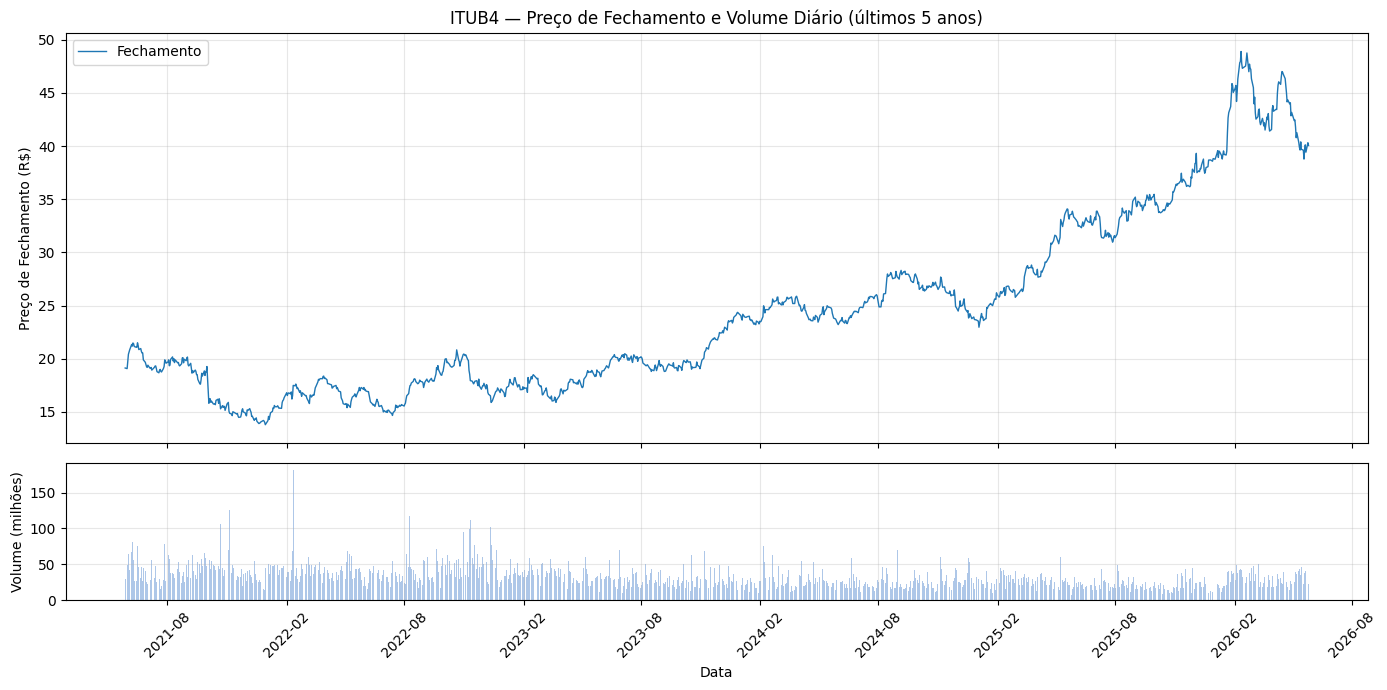
\includegraphics[width=0.95\textwidth]{figuras/01_preco_volume.png}
\caption{ITUB4 -- Preço de fechamento e volume diário no horizonte de 5 anos.}
\label{fig:precovolume}
\fonte{Elaborado pelos autores (2026).}
\end{figure}

A análise dos retornos logarítmicos diários (Figura~\ref{fig:retornos})
revela distribuição aproximadamente simétrica em torno de zero
(curtose elevada em relação à normal teórica), com caudas mais pesadas, 
comportamento típico de séries financeiras. O \textit{outlier} negativo
próximo a $-0{,}20$ corresponde ao segundo semestre de 2021, em ajuste
extraordinário do papel.

\begin{figure}[ht]
\centering
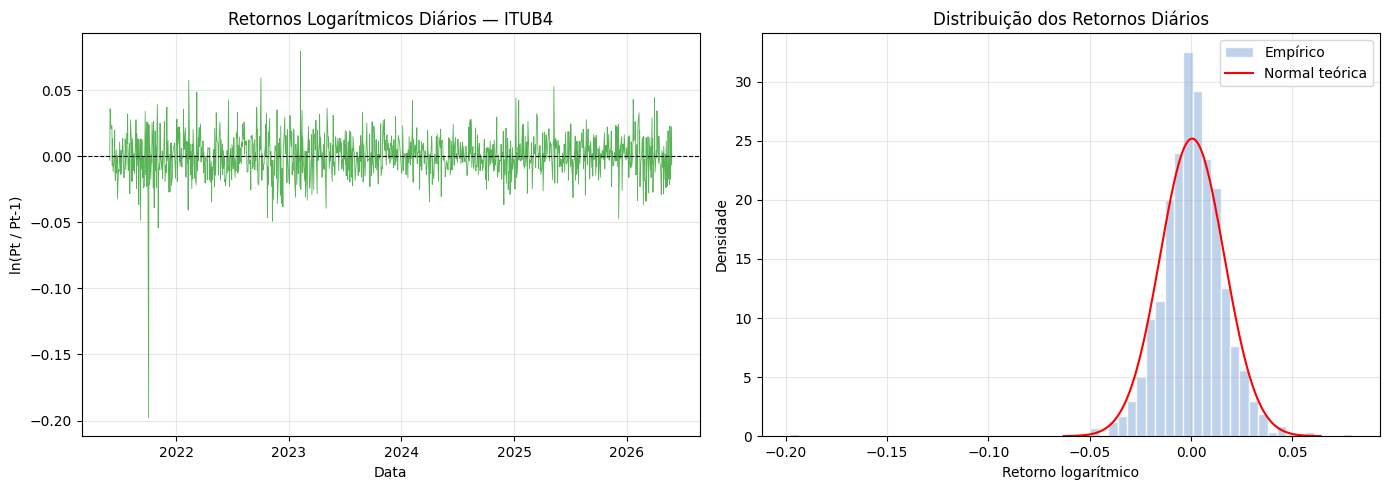
\includegraphics[width=0.95\textwidth]{figuras/02_retornos.png}
\caption{Retornos logarítmicos diários do ITUB4 e respectiva distribuição empírica.}
\label{fig:retornos}
\end{figure}

A sobreposição das médias móveis simples (SMA-20 e SMA-50) e exponencial
(EMA-60) sobre o preço de fechamento (Figura~\ref{fig:mediasmoveis})
confirma que a EMA-60 captura a tendência de médio prazo com maior
estabilidade do que as SMAs, justificando seu uso como \textit{feature}
adicional.

\begin{figure}[ht]
\centering
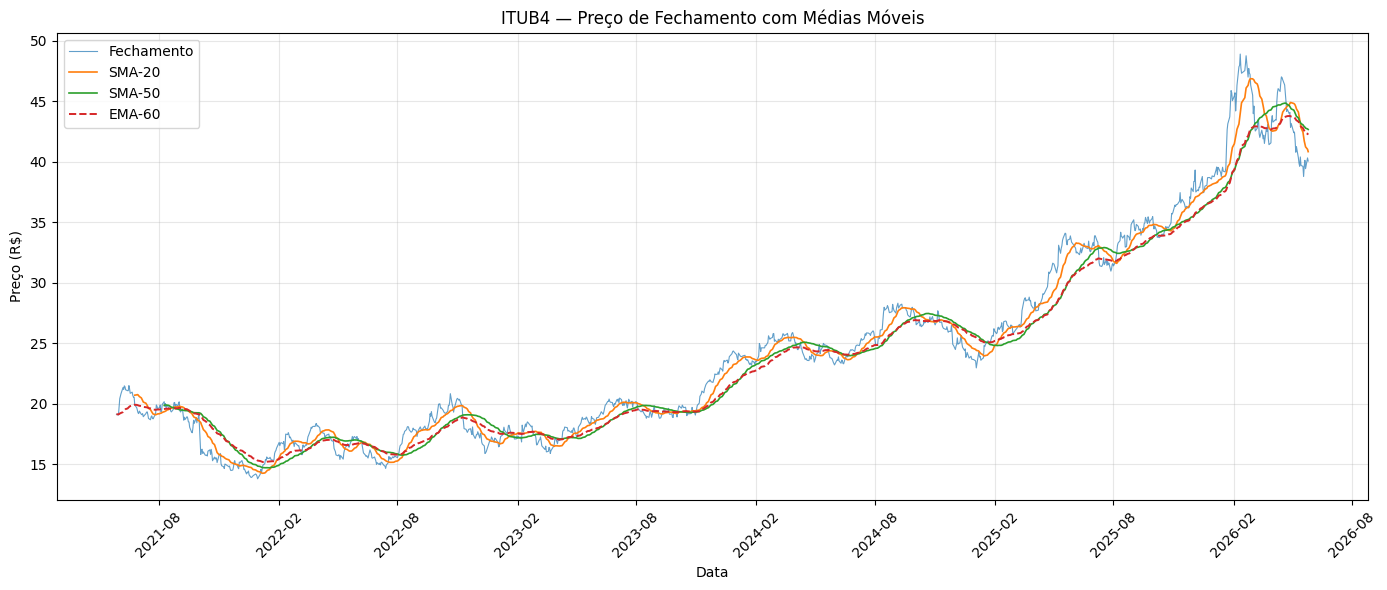
\includegraphics[width=0.95\textwidth]{figuras/03_medias_moveis.png}
\caption{Preço de fechamento do ITUB4 com sobreposição das médias móveis SMA-20, SMA-50 e EMA-60.}
\label{fig:mediasmoveis}
\end{figure}

O mapa de calor de correlação de Pearson (Figura~\ref{fig:correlacao})
indica forte multicolinearidade entre Open, High, Low, Close e EMA-60
(todas com $\rho > 0{,}985$), enquanto o Volume apresenta correlação
negativa moderada com os preços (entre $-0{,}330$ e $-0{,}343$). O padrão
é consistente com séries de preços de ativos líquidos e reforça o papel
diferenciado do volume entre as \textit{features} preditoras.

\begin{figure}[ht]
\centering
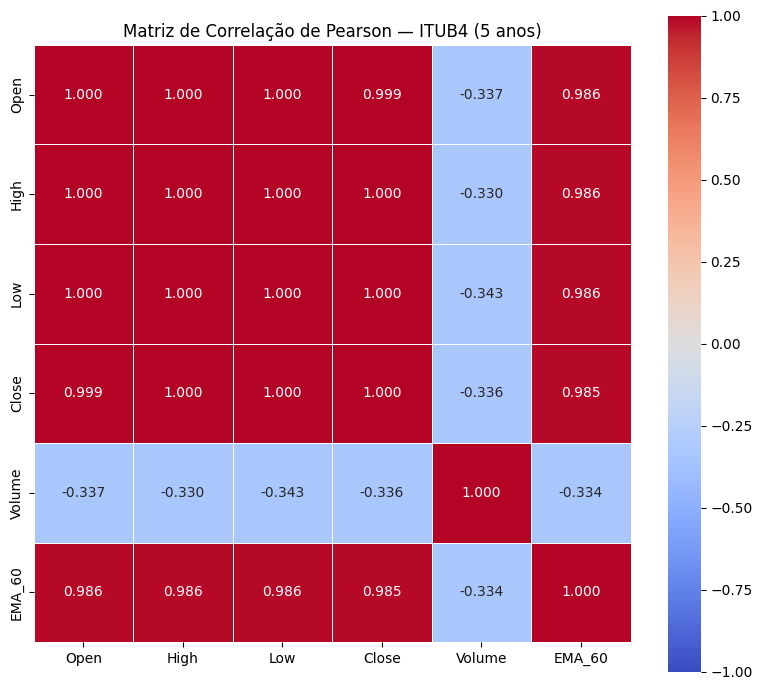
\includegraphics[width=0.65\textwidth]{figuras/04_correlacao.png}
\caption{Matriz de correlação de Pearson entre as variáveis de entrada do modelo.}
\label{fig:correlacao}
\fonte{Elaborado pelos autores (2026).}
\end{figure}

\subsubsection{Pré-processamento e Divisão Temporal}

Após o tratamento de valores ausentes via interpolação linear, a inclusão
do retorno logarítmico do fechamento como variável-alvo e a remoção da
linha inicial (defasagem), o \textit{dataset} resultou em 1.244 observações
e sete variáveis. A divisão cronológica em 80\%/20\% gerou
\textbf{995 dias para treino} (31/05/2021 a 27/05/2025) e
\textbf{249 dias para teste} (28/05/2025 a 26/05/2026).

Adotou-se o retorno logarítmico do fechamento como variável-alvo, em
substituição ao preço absoluto. Essa
escolha estabiliza a variância da série, aproxima a distribuição da
hipótese de normalidade e mitiga o risco de o modelo aprender
prioritariamente a tendência de nível em detrimento da dinâmica de
variação. A reversão à escala de reais é feita na inferência pela relação
$\hat{P}_{t+1} = P_t \cdot e^{\hat{r}_{t+1}}$.

A normalização Z-score foi aplicada individualmente às sete \textit{features},
com $\mu$ e $\sigma$ estimados exclusivamente no conjunto de treino e
escaladores serializados via \texttt{joblib}. Após o janelamento de 50 dias,
obtiveram-se os tensores $X_{\text{train}} \in \mathbb{R}^{945 \times 50 \times 7}$
e $X_{\text{test}} \in \mathbb{R}^{199 \times 50 \times 7}$.

\subsubsection{Modelo \textit{Baseline} de Persistência}

O \textit{baseline} de persistência foi avaliado sobre as 199 amostras do
conjunto de teste, no período de 07/08/2025 a 26/05/2026. As métricas
obtidas estão registradas na Tabela~\ref{tab:baseline}.

\begin{table}[ht]
\centering
\caption{Métricas do \textit{baseline} de persistência no conjunto de teste (199 amostras)}
\label{tab:baseline}
\begin{tabular}{lr}
\toprule
\textbf{Métrica} & \textbf{Valor} \\
\midrule
RMSE  & R\$ 0,6227 \\
MAE   & R\$ 0,4705 \\
MAPE  & 1,1652\% \\
\bottomrule
\end{tabular}
\fonte{Elaborado pelos autores (2026).}
\end{table}

O MAPE de aproximadamente 1,17\% indica que o \textit{benchmark} trivial
``amanhã~$=$~hoje'' incorre em erro relativo modesto, em parte explicado
pela baixa amplitude relativa das variações diárias do ativo no período
considerado. A Figura~\ref{fig:baseline} mostra a sobreposição entre preço
real e previsão do \textit{baseline}; a Figura~\ref{fig:residuosbaseline}
apresenta a distribuição dos resíduos, que se mostra centrada em zero e
sem viés sistemático visível.

\begin{figure}[ht]
\centering
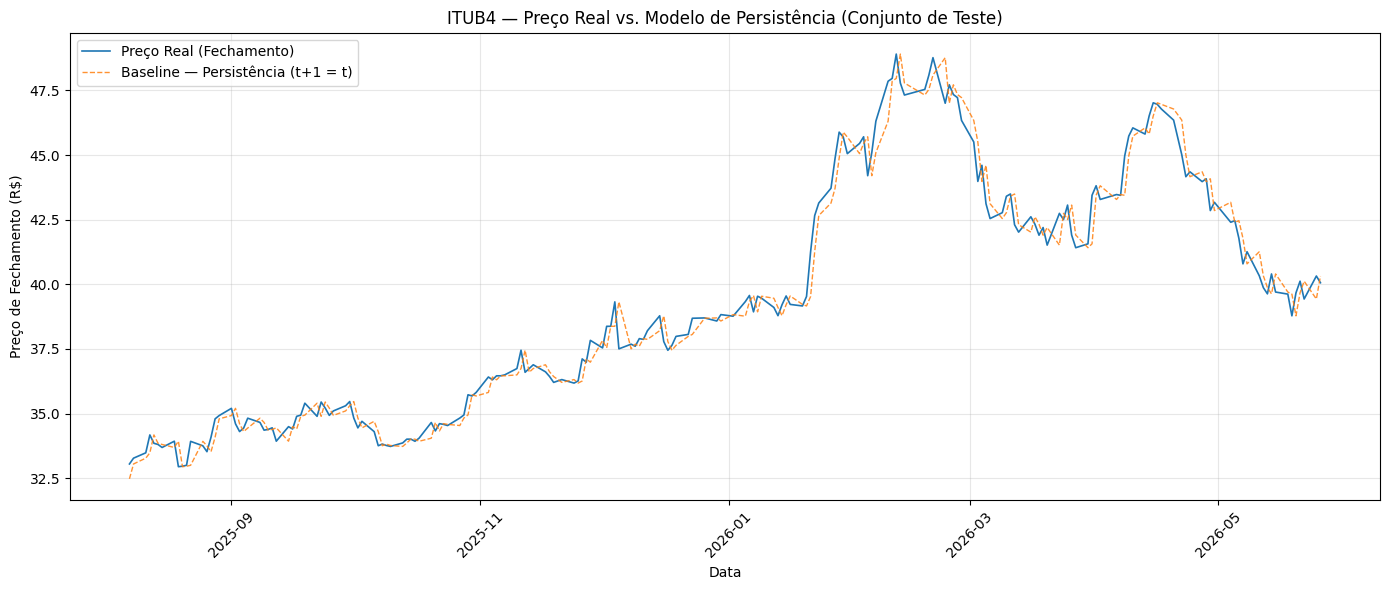
\includegraphics[width=0.95\textwidth]{figuras/05_baseline_vs_real.png}
\caption{Preço real vs.\ previsão do \textit{baseline} de persistência no conjunto de teste.}
\label{fig:baseline}
\fonte{Elaborado pelos autores (2026).}
\end{figure}

\begin{figure}[ht]
\centering
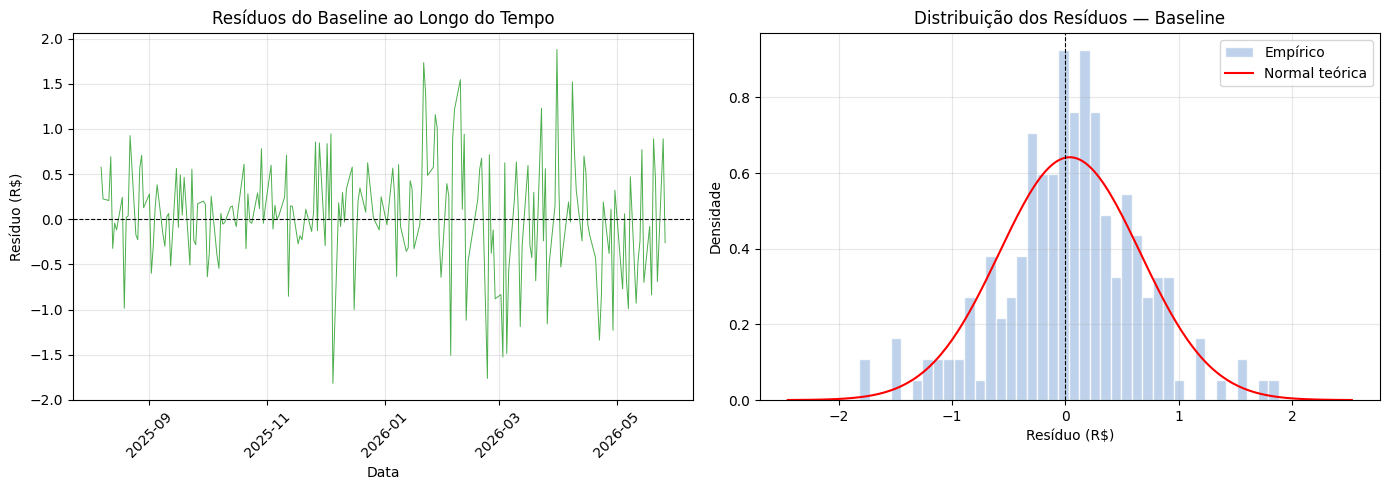
\includegraphics[width=0.95\textwidth]{figuras/06_baseline_residuos.png}
\caption{Resíduos do \textit{baseline} de persistência: série temporal e distribuição empírica.}
\label{fig:residuosbaseline}
\fonte{Elaborado pelos autores (2026).}
\end{figure}

\subsubsection{Treinamento Preliminar da LSTM}

Em sequência, foi treinada a primeira versão do modelo LSTM com a
arquitetura especificada na Tabela~\ref{tab:arq} (94.951 parâmetros
treináveis). O treinamento empregou \textit{batch size} de 32, limite de
150 épocas, fração de validação de 10\% e os \textit{callbacks}
\textit{Early Stopping} (paciência 10) e \textit{ModelCheckpoint}. A
interrupção automática ocorreu na 12ª época, com restauração dos pesos da
2ª época, na qual se observou a menor perda de validação
($\text{MSE}_{\text{val}} = 0{,}6784$ em espaço normalizado).

\begin{figure}[ht]
\centering
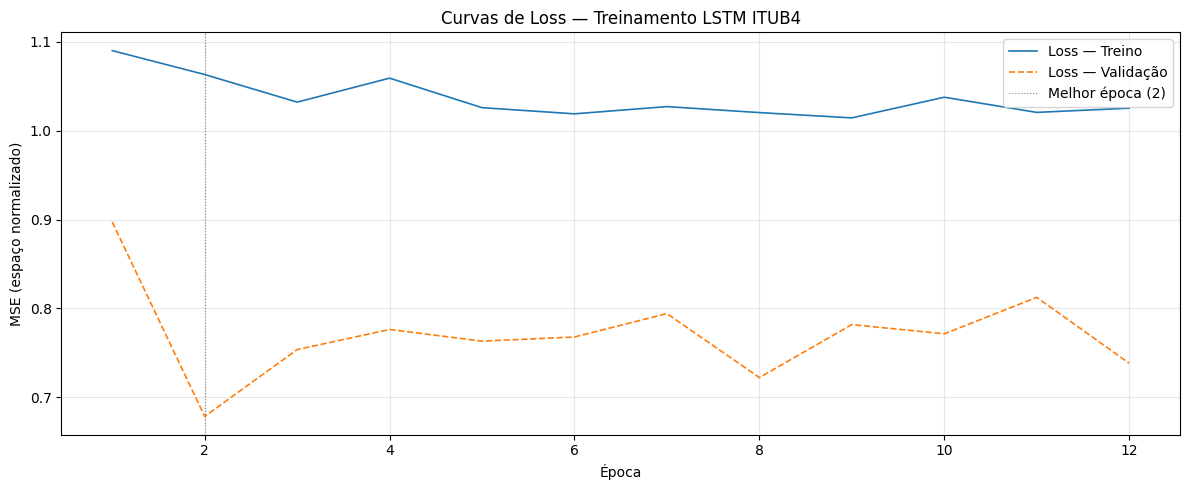
\includegraphics[width=0.95\textwidth]{figuras/07_loss.png}
\caption{Curvas de \textit{loss} de treino e validação ao longo das épocas.}
\label{fig:loss}
\fonte{Elaborado pelos autores (2026).}
\end{figure}

Aplicada ao conjunto de teste, a LSTM apresentou as métricas registradas
na Tabela~\ref{tab:comparativo}, em comparação direta com o
\textit{baseline}.

\begin{table}[ht]
\centering
\caption{Comparativo \textit{baseline} vs.\ LSTM preliminar no conjunto de teste}
\label{tab:comparativo}
\begin{tabular}{lrrr}
\toprule
\textbf{Métrica} & \textbf{Baseline} & \textbf{LSTM} & \textbf{Variação} \\
\midrule
RMSE  & R\$ 0,6227  & R\$ 0,6293  & $-1{,}06\%$ \\
MAE   & R\$ 0,4705  & R\$ 0,4719  & $-0{,}30\%$ \\
MAPE  & 1,1652\%    & 1,1703\%    & $-0{,}44\%$ \\
\bottomrule
\end{tabular}
\end{table}

As Figuras~\ref{fig:lstmreal} e~\ref{fig:comparativo} apresentam,
respectivamente, a sobreposição da previsão da LSTM com o preço real e o
comparativo conjunto entre LSTM, \textit{baseline} e valores observados.
A análise dos resíduos da LSTM (Figura~\ref{fig:residuoslstm}) revela
distribuição centrada em zero e dispersão comparável à do \textit{baseline},
sem viés sistemático aparente.

\begin{figure}[ht]
\centering
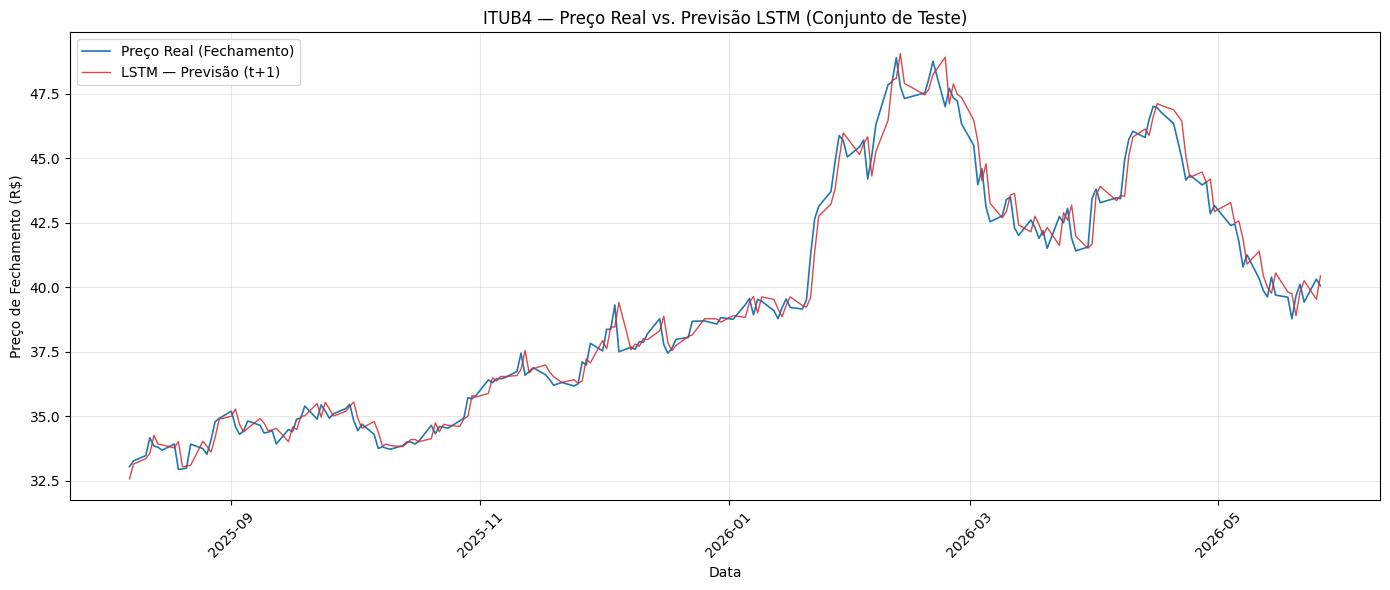
\includegraphics[width=0.95\textwidth]{figuras/08_lstm_vs_real.png}
\caption{Preço real vs.\ previsão da LSTM preliminar no conjunto de teste.}
\label{fig:lstmreal}
\end{figure}

\begin{figure}[ht]
\centering
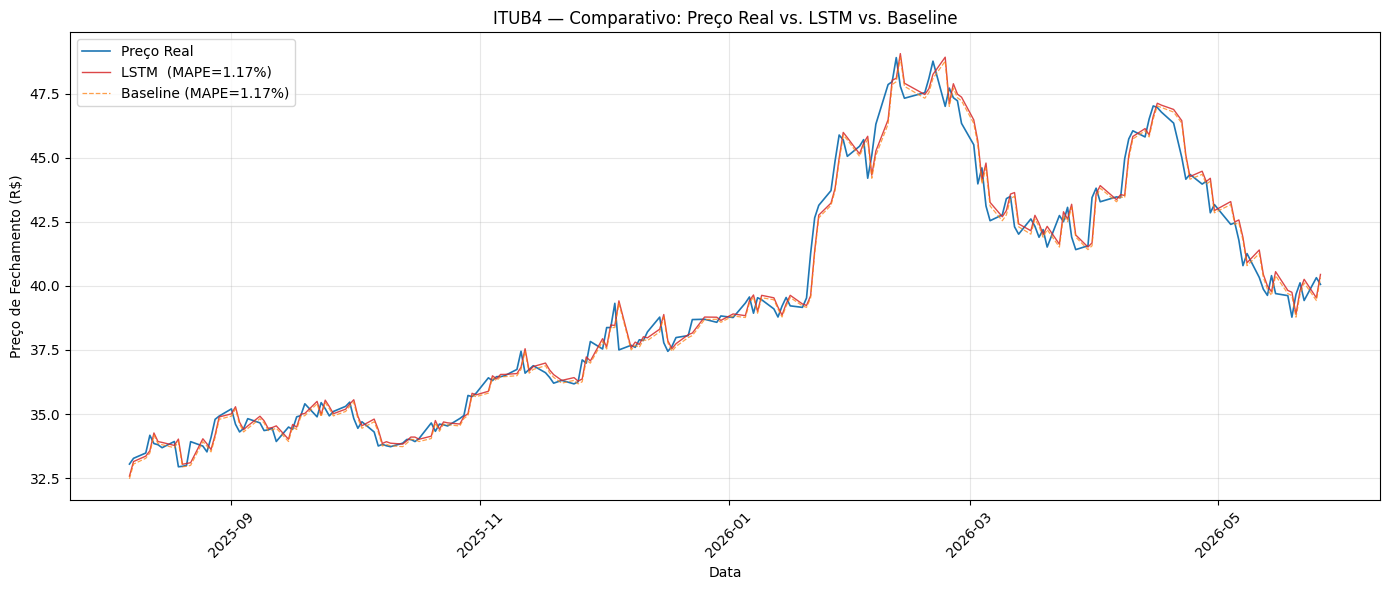
\includegraphics[width=0.95\textwidth]{figuras/09_lstm_vs_baseline.png}
\caption{Comparativo entre preço real, LSTM e \textit{baseline} no conjunto de teste.}
\label{fig:comparativo}
\end{figure}

\begin{figure}[ht]
\centering
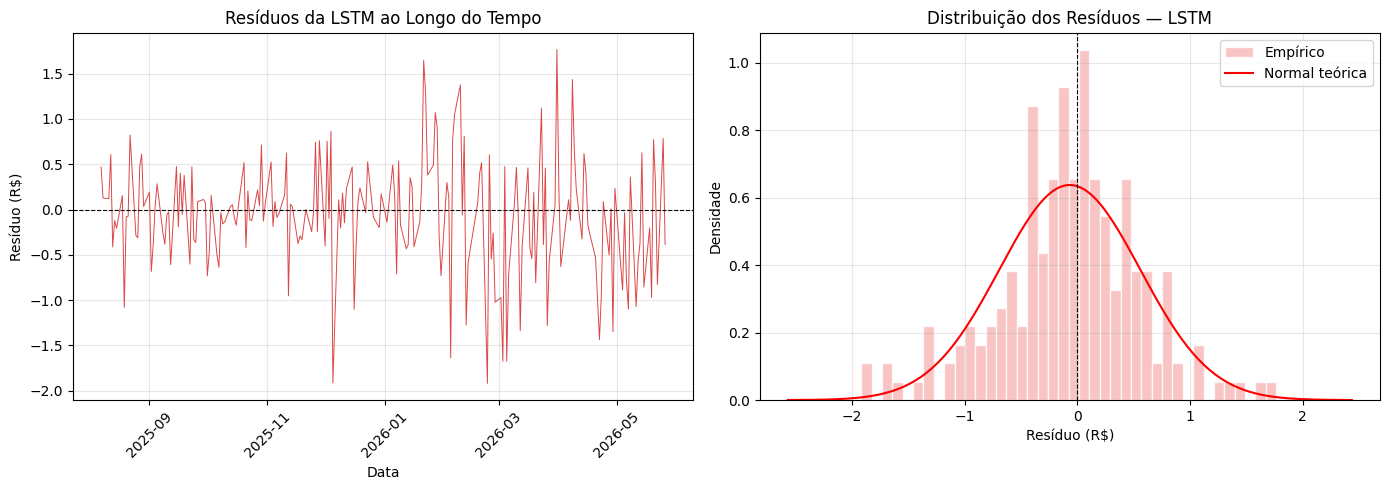
\includegraphics[width=0.95\textwidth]{figuras/10_lstm_residuos.png}
\caption{Resíduos da LSTM: série temporal e distribuição empírica.}
\label{fig:residuoslstm}
\end{figure}

\subsubsection{Discussão dos Resultados Obtidos}

Os resultados obtidos evidenciam que, na configuração atual, a LSTM
\textbf{não superou} o \textit{baseline} de persistência em nenhuma das
três métricas avaliadas. A diferença é pequena em magnitude (inferior a
1,1\% em RMSE) e provavelmente compatível com ruído de amostragem, mas o
achado é metodologicamente relevante: confirma a necessidade de iterar
sobre a configuração do modelo antes da entrega final e sustenta a
abordagem disciplinada de exigir que a LSTM supere o piso trivial
estabelecido pela persistência.

Três hipóteses orientam a próxima fase de ajuste:

\begin{itemize}
  \item \textbf{Convergência precoce:} a melhor época foi a segunda, com
        estagnação subsequente da perda de validação. Estratégias de
        redução do \textit{learning rate}, uso de \textit{schedulers}
        adaptativos e revisão do tamanho do \textit{batch} serão avaliadas;
  \item \textbf{Característica da variável-alvo:} prever o retorno
        logarítmico diário é tarefa intrinsecamente ruidosa em ativos de
        baixa volatilidade relativa. A reavaliação do alvo (preço normalizado
        direto, ou retorno suavizado) e do horizonte de previsão integrará
        a próxima iteração;
  \item \textbf{Capacidade do modelo:} a arquitetura de 150 neurônios em
        camada única pode estar superdimensionada para o sinal disponível
        em 5 anos de pregões. Configurações com menor número de unidades,
        \textit{learning rate} reduzido e regularização adicional serão
        exploradas para verificar ganho de generalização.
\end{itemize}

A inspeção visual das Figuras~\ref{fig:lstmreal} e~\ref{fig:comparativo}
sugere que a LSTM aprendeu, em essência, a reproduzir o comportamento de
persistência, com leve defasagem em transições abruptas. Esse padrão é
consistente com a hipótese de convergência precoce e direciona as próximas
iterações da Fase~3 antes da consolidação da entrega final.

\subsubsection{Protótipo Web em Streamlit}

Em paralelo à modelagem, foi desenvolvido o protótipo \textit{web} previsto
na Fase~4 da metodologia, implementado em Streamlit e organizado no
diretório \texttt{src/app/} do repositório (módulos \texttt{app.py} e
\texttt{utils.py}). A aplicação consome diretamente os artefatos
serializados pelos \textit{notebooks} -- previsões da LSTM
(\texttt{y\_pred\_lstm.npy}), previsões do \textit{baseline}
(\texttt{y\_pred\_baseline.npy}), valores reais (\texttt{y\_test\_real.npy}),
índice temporal (\texttt{test\_dates.npy}) e arquivos JSON de métricas --,
garantindo coerência integral entre os resultados reportados neste
documento e a interface apresentada ao usuário final.

A interface implementa os três blocos exigidos pela especificação original:
(i) gráfico interativo em Plotly sobrepondo preço real, previsão da LSTM e
\textit{baseline} de persistência sobre o período de teste, com
\textit{tooltips} formatadas em reais e datas em padrão brasileiro;
(ii) painel comparativo de métricas (RMSE, MAE, MAPE) apresentado em
\textit{cards} numéricos individuais e em tabela consolidada, com indicação
explícita da variação percentual da LSTM em relação ao \textit{baseline};
e (iii) seção obrigatória de aviso legal e limitações, em conformidade com
os aspectos éticos discutidos na Subseção~4.1. A Figura~\ref{fig:streamlit}
apresenta a tela inicial da aplicação em execução.

\begin{figure}[ht]
\centering
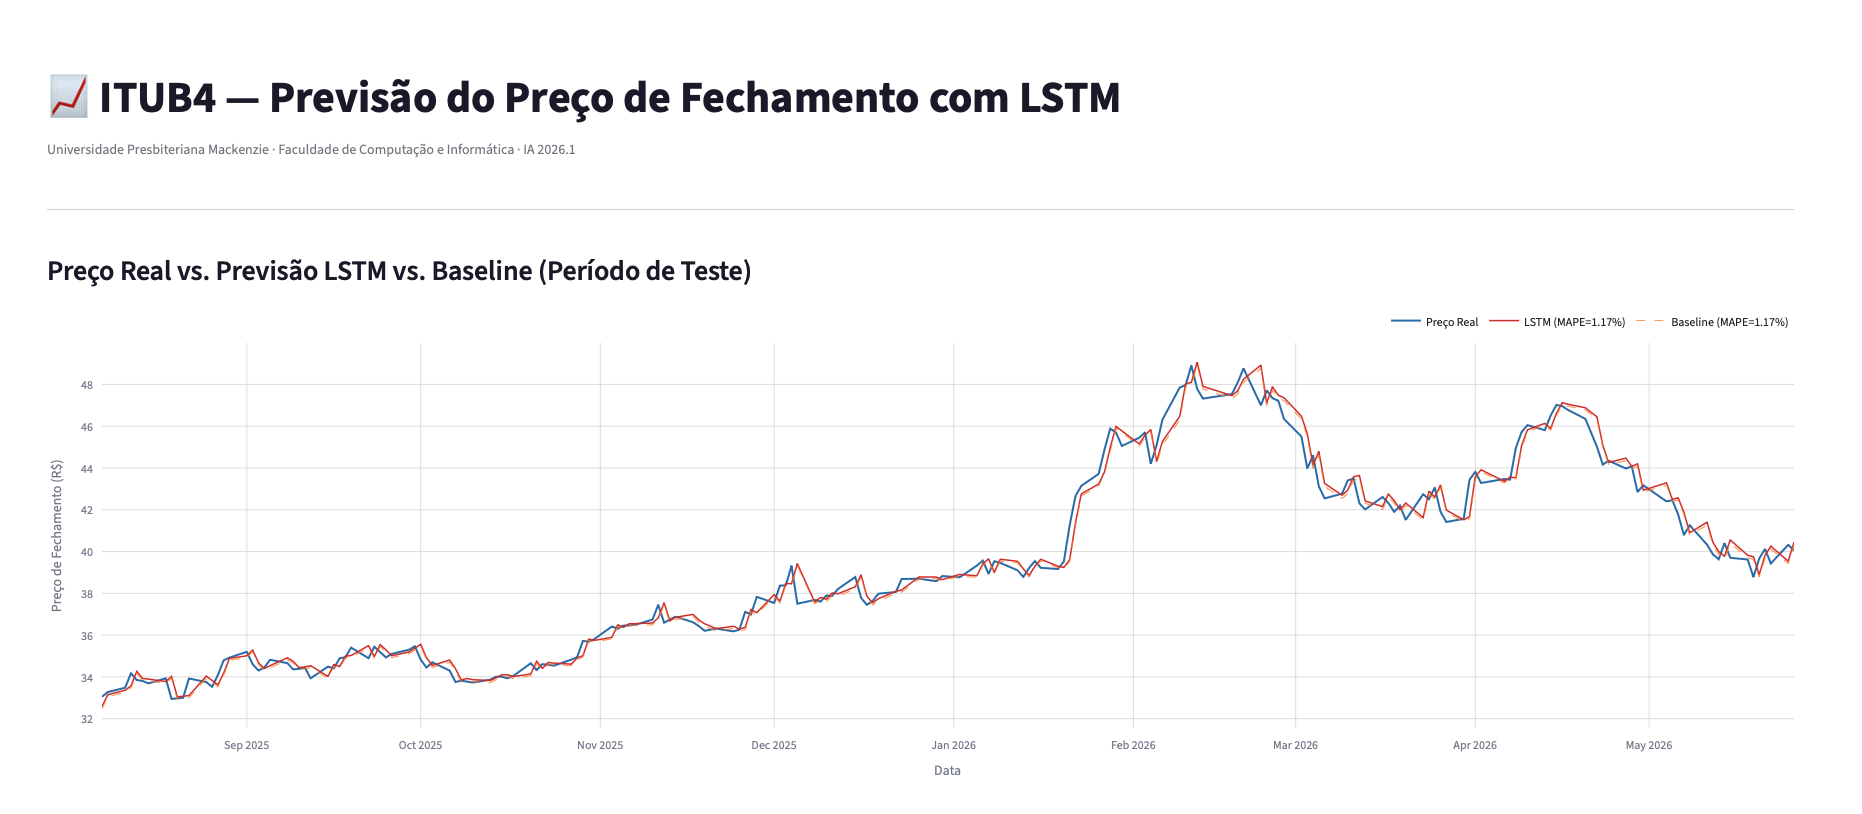
\includegraphics[width=0.95\textwidth]{figuras/11_streamlit_app.png}
\caption{Tela inicial do protótipo Streamlit -- gráfico comparativo entre preço real, LSTM e \textit{baseline} no período de teste.}
\label{fig:streamlit}
\end{figure}

Um painel expansível de ``Detalhes do Modelo'' descreve os
hiperparâmetros, \textit{features}, janela temporal, normalização e
otimizador empregados, oferecendo ao usuário a rastreabilidade técnica
necessária para interpretar criticamente as previsões. O aviso legal --
\textit{``Esta ferramenta é um apoio analítico baseado em padrões
históricos. O desempenho passado não garante resultados futuros. Não
constitui recomendação de investimento.''} é apresentado em destaque
imediatamente após o painel de métricas, seguido da seção de limitações
técnicas que explicita a incapacidade do modelo de incorporar eventos
exógenos, análise fundamentalista, sentimento de mercado e horizontes de
previsão superiores a um dia útil.

A entrega do protótipo \textit{web} cumpre o objetivo específico definido
na Subseção~1.3 e completa a infraestrutura prevista para a entrega final.
As próximas iterações concentram-se exclusivamente no ajuste do modelo
LSTM, sem necessidade de reescrita da camada de apresentação, bastando
a substituição dos artefatos serializados quando a nova versão do modelo
superar o \textit{baseline}.

\subsection{Repositório GitHub}

O código-fonte, os \textit{notebooks} de análise exploratória e os artefatos
gerados estão disponíveis no repositório público.
Disponível em: \url{https://github.com/LucasZanini096/Artificial-Intelligence-Project}.
Acesso em: 27 maio 2026.

% ===========================================================================
\section{Considerações Finais}
% ===========================================================================

Este relatório parcial documentou as três primeiras fases do projeto de
previsão do preço de fechamento da ação ITUB4 com rede neural LSTM:
coleta e análise exploratória de cinco anos de dados via API
\textit{yfinance}, pré-processamento com normalização Z-score e janelamento
temporal de 50 dias, e uma primeira iteração de treinamento do modelo em
comparação direta com o \textit{baseline} de persistência.

A principal contribuição metodológica até o momento é a constatação,
amparada por evidência empírica, de que a configuração inicial da LSTM
(camada única, 150 neurônios, retorno logarítmico como alvo) \textbf{não
supera} o \textit{baseline} trivial em nenhuma das três métricas avaliadas
(RMSE, MAE e MAPE), com diferença inferior a 1,1\%. O achado reforça a
importância de manter o \textit{baseline} como piso obrigatório de
comparação e direciona as próximas iterações da Fase~3 para três frentes
específicas: ajuste de \textit{learning rate} e estratégia de
\textit{schedulers}, reavaliação da variável-alvo (preço normalizado direto
ou retorno suavizado) e redução da capacidade do modelo para mitigar
convergência precoce.

A entrega completa o protótipo \textit{web} previsto na Fase~4, integrando
os artefatos serializados em uma aplicação Streamlit funcional com aviso
legal e seção de limitações em conformidade com os aspectos éticos
discutidos. A camada de apresentação está estabilizada e as iterações
restantes do projeto concentram-se exclusivamente na obtenção de um modelo
LSTM cujo desempenho supere o \textit{baseline} em todas as métricas, com
meta de MAPE inferior a 2\% na entrega final.

% ===========================================================================
\bibliographystyle{sbc}
\bibliography{referencias_n1}
% ===========================================================================

\end{document}
